\documentclass[11pt,a4paper]{article}
\usepackage{tikz}
\usetikzlibrary{decorations.pathmorphing}
\usepackage{amsmath,amssymb,amsbsy,amsfonts,latexsym,graphicx}
\usepackage{color,array,subfigure}

\begin{document}

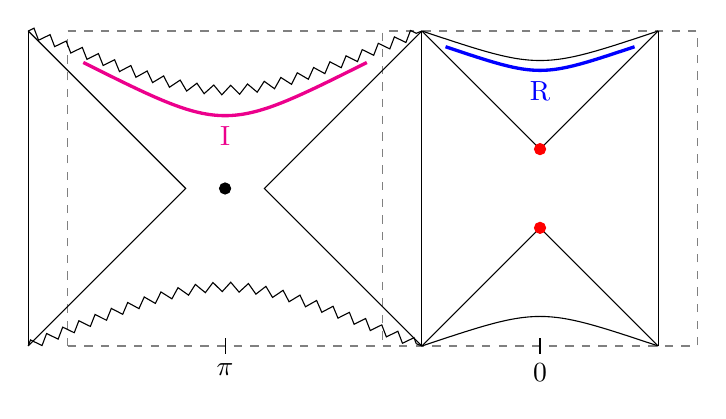
\begin{tikzpicture}
\draw [gray, dashed] (0,0) -- (0,4);
      \draw[gray, dashed] (0,4) -- (4,4)
     ;
\draw[gray, dashed] (0,0) -- (4,0)
    ;
\draw [gray, dashed] (4,0) -- (8,0) -- (8,4) -- (4,4) -- (4,0);
\draw (4.5,0) -- (4.5,4);
\draw (-0.5,0) -- (-0.5,4);
\draw (7.5,0) -- (7.5,4);
\draw [decorate,decoration={zigzag,segment length=2.2mm, amplitude=0.6mm}] (-0.5,0) .. controls (2,1) .. (4.5,0);
\draw [decorate,decoration={zigzag,segment length=2.2mm, amplitude=0.6mm}] (-0.5,4) .. controls (2,3) .. (4.5,4);
\draw  (4.5,0) .. controls (6,0.5) .. (7.5,0);
\draw  (4.5,4) .. controls (6,3.5) .. (7.5,4);
\draw [very thick, blue] (4.8,3.8) .. controls (6,3.4) .. (7.2,3.8)
node[midway, below] {R};
\draw [very thick, magenta] (0.2,3.6) .. controls (2,2.7) .. (3.8,3.6)
node[midway, below] {I};
\draw (-0.5,0) -- (1.5,2) -- (-0.5,4);
\draw (4.5,0) -- (2.5,2) -- (4.5,4);
\draw (4.5,4) -- (6,2.5) -- (7.5,4);
\draw (4.5,0) -- (6,1.5) -- (7.5,0);
\filldraw[black] (2,2) circle (2pt);
\filldraw[red] (6,2.5) circle (2pt);
\filldraw[red] (6,1.5) circle (2pt);
\draw (2,0.1)--(2,-0.1) node [below] {$\pi$};
\draw (6,0.1)--(6,-0.1) node [below] {$0$};
\end{tikzpicture}

\end{document}